\documentclass[12pt,a4paper]{article}

\usepackage[margin=1in]{geometry}
\usepackage[T1]{fontenc}
\usepackage{amsmath}
\usepackage{listings}
\usepackage{pgfplots}
\pgfplotsset{compat=1.16}

\title{Labwork 3 Report: Hello, CUDA!}
\author{Dao Quy Tung \\ Student ID: 2540109}
\date{\today}

\begin{document}

\maketitle

\section{Introduction}
This labwork converts an RGB image to grayscale using both a sequential CPU loop and a parallel CUDA kernel written with \texttt{numba.cuda}. I checked that the two implementations produce identical pixel values, measured their execution times, and examined how CUDA block size affects kernel time.

\section{Implementation}
The input is a $1200\times600$ RGB JPEG image, containing 720,000 pixels. I loaded it with \texttt{matplotlib.image.imread} and reshaped it into a \texttt{(720000, 3)} array. For each pixel, both implementations compute the integer mean of the red, green, and blue channels:
\begin{equation}
g=\left\lfloor\frac{R+G+B}{3}\right\rfloor.
\end{equation}
The value $g$ is written into all three output channels, so the saved RGB image appears grayscale.

\subsection{CPU version}
The CPU version uses a \texttt{for} loop over every pixel. It converts each channel value to a Python integer before addition and writes the result into a \texttt{uint8} output array.

\subsection{CUDA version}
The CUDA kernel assigns one thread to each pixel. It computes the global thread index from the block and thread indices, checks the array boundary, and writes the grayscale value:

\begin{lstlisting}[language=Python,basicstyle=\ttfamily\small,breaklines=true]
@cuda.jit
def grayscale(src, dst):
    tidx = cuda.threadIdx.x + cuda.blockIdx.x * cuda.blockDim.x
    if tidx < src.shape[0]:
        r = int(src[tidx, 0])
        g = int(src[tidx, 1])
        b = int(src[tidx, 2])
        gray = np.uint8((r + g + b) // 3)
        dst[tidx, 0] = gray
        dst[tidx, 1] = gray
        dst[tidx, 2] = gray
\end{lstlisting}

The host transfers the input with \texttt{cuda.to\_device}, allocates the output with \texttt{cuda.device\_array}, launches the kernel with \texttt{grayscale[gridSize, blockSize]}, and retrieves the result with \texttt{copy\_to\_host()}. The number of blocks is \(\lceil\text{pixelCount}/\text{blockSize}\rceil\). I used 64 threads per block for the CPU--GPU timing comparison.

\section{Validation and timing results}
I saved the CPU and GPU images as \texttt{gray\_cpu.png} and \texttt{gray\_gpu.png}. The program's \texttt{np.array\_equal} check returned \texttt{True}: all output pixel values matched.

The CUDA kernel was run once before measurement so that just-in-time compilation was excluded. The GPU time below includes allocation, host-to-device transfer, kernel execution, and device-to-host transfer. Times were measured using \texttt{time.time()} on an NVIDIA GeForce RTX 2050.

\begin{center}
\begin{tabular}{lr}
\hline
Measurement & Result \\
\hline
CPU sequential loop & 0.746450 s \\
GPU full workflow & 0.003859 s \\
CPU time / GPU time & 193.43$\times$ \\
Output arrays identical & Yes \\
\hline
\end{tabular}
\end{center}

The speedup compares this Python CPU loop with the complete measured GPU workflow for this particular image. It does not include the one-time CUDA compilation cost.

\section{Effect of block size}
I tested five block sizes. For each size, the input and output arrays remained on the GPU, and I measured 30 kernel launches. Each launch was followed by \texttt{cuda.synchronize()}; the table reports the median time. These kernel-only measurements therefore have a different scope from the full GPU time above.

\begin{center}
\begin{tabular}{rr}
\hline
Threads per block & Median kernel time (ms) \\
\hline
32  & 0.1837 \\
64  & 0.1247 \\
128 & 0.1179 \\
256 & 0.1137 \\
512 & 0.1241 \\
\hline
\end{tabular}
\end{center}

\begin{figure}[htbp]
\centering
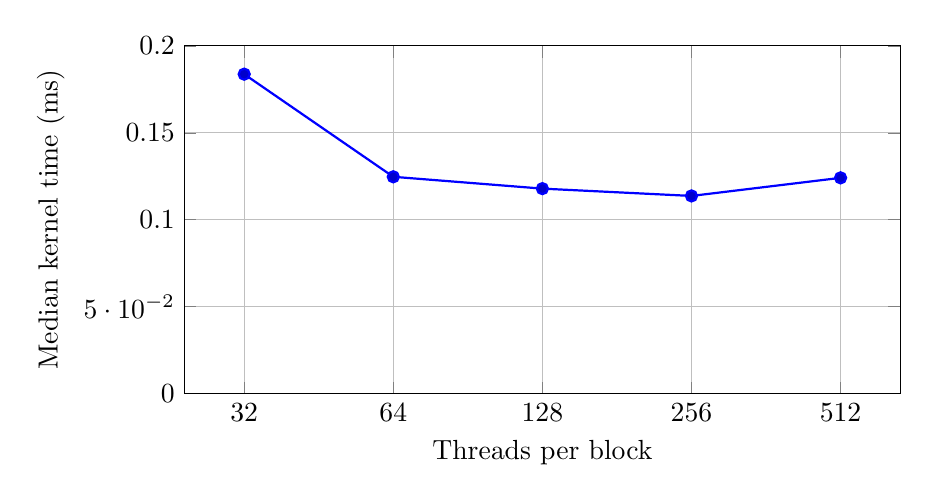
\begin{tikzpicture}
\begin{axis}[
    width=0.88\linewidth,
    height=6cm,
    xlabel={Threads per block},
    ylabel={Median kernel time (ms)},
    symbolic x coords={32,64,128,256,512},
    xtick=data,
    ymin=0,
    ymax=0.20,
    ytick={0,0.05,0.10,0.15,0.20},
    grid=major
]
\addplot+[mark=*,thick] coordinates {
    (32,0.1837) (64,0.1247) (128,0.1179)
    (256,0.1137) (512,0.1241)
};
\end{axis}
\end{tikzpicture}
\caption{Block size versus median kernel execution time.}
\end{figure}

Among the tested values, 256 threads per block gave the lowest median kernel time, 0.1137 ms. Increasing the block size from 256 to 512 did not improve this result. The differences are small in absolute time, so the best block size should be understood as the best observed in this run rather than a universal setting.

\section{Conclusion}
Both implementations produced the same grayscale image. For this 720,000-pixel input, the measured GPU workflow took 0.003859 s compared with 0.746450 s for the sequential Python loop. The block-size experiment showed that kernel time varied with launch configuration, with 256 threads per block performing best among the five values tested.

\end{document}
